\documentclass[12pt,a4paper]{article}

\usepackage[utf8]{inputenc}
\usepackage[T1]{fontenc}
\usepackage[french]{babel}

\usepackage{amsmath, amssymb}

\usepackage{graphicx}
\usepackage{caption}

\usepackage{siunitx} % Pour les unités

\usepackage{geometry}
\geometry{top=2.5cm, bottom=2.5cm, left=3cm, right=3cm}
\setlength{\parindent}{0pt}


\usepackage{enumitem}

\usepackage{hyperref}

\usepackage{xcolor}

\usepackage{multicol}
\setlength{\columnseprule}{0pt}
\def\columnseprulecolor{\color{gray}}

\usepackage{tcolorbox}


\usepackage{import}
\usepackage{xifthen}
\usepackage{pdfpages}
\usepackage{transparent}
\usepackage{float}

\newcommand{\incfig}[1]{%
	\def\svgwidth{\columnwidth}
	\import{./figures/}{#1.pdf_tex}
}


\newcommand{\RomanNum}[1] %pour les chiffre romain
{\MakeUppercase{\romannumeral #1}}




\usepackage{lipsum}















\title{Projet struture en béton armé}
\author{AMALOU Jugurta}
\date{\today}

\begin{document}
	\counterwithin{section}{part} % pour que \section{} recommence de 1 aprés \part{}
	
	
	\tableofcontents
	
	\newpage
	
	\part{Chapitre \RomanNum{1}}
	
	
	
	
	\section{Présentation et descrpition de l'ouvrage}
	
	
	
	
	\section{Caractéristique des matériaux}
	
	
	
	
	
	\section{Pré-dimensionnement}
	
	\textbf{Le pré-dimensionement se fait a l'ELS}
	
	
	
	
	\subsection{Pré-dimensionnement du plancher}
	
	
	
	
	\[ H_{p} = \dfrac{L_{\max}}{22,5} \]
	
	Avec :
	
	$H_{p}$ : la hauteur du plancher.
	
	$L_{\max}$ : La plus grande travée (plus grande distance entre nus d'appuies).
	
	
	
	\[ \begin{cases}
		\text{si  } H_{p} < 16+4 = 20~\unit{cm} \text{  alors on choisie un plancher en 16+4} \\\\
		\text{sinon si  } 16+4 < H_{p} < 20+5 \text{  alors on va opter pour un plancher en 25 cm} 
	\end{cases} \]
	
	\[ L_{\max} = 4,4~\unit{m}  \]
	
	\[ H_{p} = \dfrac{440}{22,5} = 19,55~\unit{cm} < 20~\unit{cm} \]
	
	\fbox{On va opter pour un plancher en corps-creux de $16+4 = 20~\unit{cm}$.}
	
	
	
	
	\subsection{Pré-dimensionnement des poutres}
	
	
	
	
	
	
	
	\subsubsection{Hauteur de la poutre}
	
	\[ \dfrac{L_{\max}}{15} < h < \dfrac{L_{\max}}{10} \]
	
	
	
	\[ L_{\max} = 4,4~\unit{m} \]
	
	\[ 29,33~\unit{cm} < h < 44~\unit{cm} \]
	
	et selon le RPA on a $h \geq 30~\unit{cm}$
	
	
	
	On choisie $h = 35~\unit{cm}$
	
	
	

	
	
	
	\subsubsection{Largeur de la poutre}
	
	
	
	\[ 0,4 \cdot h \leq b \leq 0,7 \cdot h \]
	
	
	Avec $h$ étant la hauteur de la poutre.
	
	\[
	\begin{aligned}
		0,4 \cdot 35 \leq &b \leq 0,7 \cdot 35 \\
		14 \leq &b \leq 24,5
	\end{aligned}  
	\]
	
	Selon le RPA on $b \geq 20~\unit{cm}$
	
	On choisie : $b = 25~\unit{cm}$
	
	\vspace{\baselineskip}
	
	\[ \text{Pour éviter un déversement selon le RPA on a :} \quad \dfrac{h}{b} \leq 4 \longrightarrow 1,4 < 4 \text{ Condition vérifier} \]
	
	
	
	
	\[\begin{aligned}
		 b_{\max} &\leq 1,5 \cdot h + b \\
		 b_{\max} &\leq 1,5 \cdot 35 + 25 \\
		 b_{\max} &\leq 77,5
	\end{aligned}\]
	
	
	\subsubsection{Dimensions retenues de la poutre}
	
	On opte finalement pour :
	
	\[ \fbox{$h = 35~\unit{cm} \quad;\quad b = 25~\unit{cm}$} \]
	
	
	
	
	
	
	
	\subsection{Pré-dimensionnement des voiles}
	
	
	\[ e = \dfrac{h_{e}}{20} \]
	
	Avec $h_{e}$ étant la hauteur d'étage libre.
	
	
	\vspace{\baselineskip}
	
	Et selon le RPA : 
	
	\[ e_{min} = 15~\unit{cm} \]
	
	\vspace{\baselineskip}
	
	\begin{multicols}{2}
	
	\subsubsection{Étage courant}
	
	\[ h_{e} = 323 - 20 = 303~\unit{cm} \]
	
	\[ e = \dfrac{303}{20} = 15,15~\unit{cm} \]
	
	\columnbreak
	
	\subsubsection{RDC}
	
	\[ h_{e} = 408-20 = 388~\unit{cm} \]
	
	\[ e = \dfrac{388}{20} = 19,4~\unit{cm} \]

	
	\end{multicols}
	
	\vspace{\baselineskip}
	
	Finalement on opte pour les deux cas \fbox{$e = 20~\unit{cm}$}
	
	
	\vspace{\baselineskip}
	
	
	\subsection{Pré-dimensionnement des pouteaux}
	
	On dimensionne uniquement le poteau le plus solicité. Et ce dernier est celui qui reprend le plus de surface.
	
	
	
	
	
	
	\begin{figure}
		\centering
		\includegraphics[width=0.7\linewidth]{"figures/plancher reprie par poteau"}
		\caption{}
		\label{fig:plancher-reprie-par-poteau}
	\end{figure}
	
	
	
	
	
	
	
	
	

	
	\subsubsection{Calcul decente des charges}
	
	
	
	\paragraph{Plancher terrasse inaccessible} : 
	
	
	Charges permanentes :
	
	\begin{itemize}
		\item Enduit platre = $0,2~\unit{kN\per m^{2}}$
		\item Hourdis + Dalle de copression = $2,8~\unit{kN\per m^{2}}$
		\item Isolation thermique = $0,16~\unit{kN\per m^{2}}$
		\item Feuille de polyne = $0,01~\unit{kN\per m^{2}}$
		\item Forme de pente en béton = $1,54~\unit{kN\per m^{2}}$
		\item Feuille de pax (étanchiéter multi couche) = $0,12~\unit{kN\per m^{2}}$
		\item Couche de gravier = $0,85~\unit{kN\per m^{2}}$
	\end{itemize}
	
	\[ g = 0,2+2,8+0,16+0,01+... = 5,68~\unit{kN\per m^{2}} \]
	
		
	Charges d'exploitation : $q = 1~\unit{kN\per m^{2}}$
	
	
	Poids volumique du béton armé : $\rho_{ba} = 25~\unit{kN\per m^{3}}$
	
	\vspace{2\baselineskip}
	
	
	
	\begin{itemize}
		\item Charge permanente du plancher :
		\[
		\begin{aligned}
			G_{plancher} &= 5,68 \cdot  \bigg( (2,275 + 2,225) \cdot (1,475 + 2,148) \bigg) \\
			&=92,6~\unit{kN}
		\end{aligned}
		\]
		
		\item Poids propre des poutres : 
		\[
		\begin{aligned}
			G_{poutres} &= 25 \cdot \bigg( 0,25 \cdot \bigg( (1,475+2,148) + (2,275 + 2,225) \bigg) \bigg) \\
			&= 50,77~\unit{kN}
		\end{aligned}
		\]
		
		\item Poids propre du poteau :
		
		\[
		G_{poteau} = 25 \cdot (0,3 \cdot 0,4 \cdot 3,23) = 9,69~\unit{kN}
		\]
		
		\item Surcharge d'exploitation : 
		
		\[ Q = 1 \cdot 4,75 \cdot 3,87 = 18,38~\unit{kN} \]
	\end{itemize}
	
	
	
	
	finalement pour le plancher terrasse on aura : 
	
	\[ G = 92,6 + 50,77 + 9,69 = 153,06~\unit{kN} \]
	
	\[ Q = 18,38~\unit{kN} \]
	
	\[ \fbox{$F = G + Q = 171,44~\unit{kN} $}\]
	
	
	
	
	
	
	\paragraph{Plancher courant} :
	
	Charges permanentes :
	
		\begin{itemize}
		\item Enduit = $0,4~\unit{kN\per m^{2}}$
		\item Hourdis + Dalle de copression = $2,8~\unit{kN\per m^{2}}$
		\item Cloison en brique = $0,9~\unit{kN\per m^{2}}$
		\item Isolation phonique = $0,1~\unit{kN\per m^{2}}$
		\item Couche de sable = $0,36~\unit{kN\per m^{2}}$
		\item Mortier de pose = $0,44~\unit{kN\per m^{2}}$
		\item Carrelage = $0,4~\unit{kN\per m^{2}}$
	\end{itemize}
	
	\[ g = 0,4 + 2,8 + 0,9 + 0,1 +... = 5,4~\unit{kN\per m^{2}} \]
	
	Charges d'exploitation : $q = 1,5~\unit{kN\per m^{2}}$
	
	
	Poids volumique du béton armé : $\rho_{ba} = 25~\unit{kN\per m^{3}}$
	
	
	\vspace{2\baselineskip}
	
	
	
	
	\begin{itemize}
		\item Charge permanente du plancher :
		\[
		G_{planche} = 16,3~\unit{m^{2}} \cdot 5,4 = 88,02~\unit{kN}
		\]
		
		\item Poids propre des poutres : 
		\[
		G_{poutres} = 50,77~\unit{kN}
		\]
		
		\item Poids propre des poteaux couratns :
		
		\[
		G_{poteau} = 25 \cdot (0,3 \cdot 0,4 \cdot 3,23) = 9,69~\unit{kN}
		\]
		
		\item Poids propre du poteau du RDC :
		
		\[ G_{poteauRDC} = 25 \cdot (0,3 \cdot 0,4 \cdot 4,08) = 12,24~\unit{kN} \]
		
		\item Surcharge d'exploitation : 
		
		\[ Q = 1,5 \cdot 4,75 \cdot 3,87 = 27,57~\unit{kN} \]
	\end{itemize}
	
	\vspace{2\baselineskip}
	
	
	
	\[ G = 88,02 + 50,77 + 9,69 = 148,48~\unit{kN} \]
	
	\[ G_{RDC} = 88,02 + 50,77 + 12,24 = 151,03~\unit{kN} \]
	
	
	
	\vspace{\baselineskip}
	
	\[ \fbox{$F = G+Q = 148,48 + 27,57 =176,05~\unit{kN} $} \]
	
	\[ \fbox{$F_{RDC} = G_{RDC} + Q = 151,03 + 27,57 = 178,6~\unit{kN}$} \]

	
	
	
	
	
	\begin{figure}[H]
		\centering
		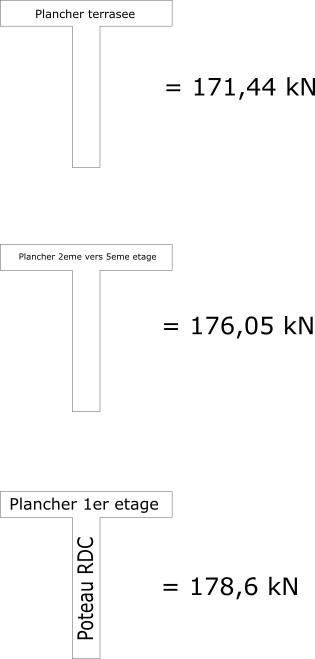
\includegraphics[width=0.5\linewidth]{figures/charge-des-planchers}
		\caption{Les poids selon les étages}
		\label{fig:charge-des-planchers}
	\end{figure}
	
	\vspace{2\baselineskip}
	
	\subsubsection{Calculs des sections des poteaux}
	
	
	\[ \sigma = \dfrac{F}{S} \quad\leq\quad \overline{\sigma}_{b} = 0,6 \cdot f_{c28} \]
	
	\[ \downarrow \]
	
	\[ S \geq \dfrac{F}{\overline{\sigma}_{b}} \]

	
	Avec S étant la section du poteau et $\overline{\sigma}_{b} = 0,6 \cdot 25~\unit{MPa} =  15 \cdot 10^{3}~\unit{kN\per m^{2}}$
	
	\vspace{\baselineskip}
	
	D'aprés le RPA les dimension minimale selon les zones sismiques sont : 
	
	\begin{equation}
		\begin{split}
			\min(a, b) &\geq 25~\unit{cm} \text{  en zones 	$\RomanNum{1}$ et $\RomanNum{2}$a } \\
			\min(a, b) &\geq 30~\unit{cm} \text{  en zones 	$\RomanNum{2}$b et $\RomanNum{3}$}
		\end{split}
		\label{dtr:RPA prédimensionnement poutre}
	\end{equation}
	
	
	
	\paragraph{Poteaux du RDC, $1^{er}$ et $2^{eme}$ étages} :
	
	Le plus solicité est le poteau du RDC : 
	
	\[ F = 171,44 + 4 \cdot 176,05 + 178,6 = 1054,25~\unit{kN} \]
	
	
	
	
	
	\[ S \geq \dfrac{1054,25}{15000} = 0,0703~\unit{m^{2}} = 703~\unit{cm^{2}} \]
	
	On considerant les section minimale imposée par le RPA (25 cm) on aura :
	
	\[ a \cdot 25 \geq 703 \longrightarrow a \geq 28,12~\unit{cm} \]
	
	Finalement : \[\fbox{$ a = 30~\unit{cm} \quad ; \quad b = 25~\unit{cm} $}\]
	
	
	\vspace{5\baselineskip}
	
	
	
	\paragraph{Poteaux du $3^{er}$ jusqu'a la terrasse} :
	
	Le plus solicité est le poteau du $3^{eme}$ étage : 
	
	\[ F = 171,44 + 2 \cdot 176,05 = 523,54~\unit{kN} \]
	
	
	
	
	
	\[ S \geq \dfrac{525,54}{15000} = 0,034~\unit{m^{2}} = 340~\unit{cm^{2}} \]
	
	On considerant les section minimale imposée par le RPA (25 cm) on aura :
	
	\[ a \cdot 25 \geq 340 \longrightarrow a \geq 13,6~\unit{cm} \]
	
	Finalement : \[\fbox{$ a = 25~\unit{cm} \quad ; \quad b = 25~\unit{cm} $}\]
	
	
	
	
\end{document}